\NeedsTeXFormat{LaTeX2e}
\documentclass[a4paper,12pt,
headsepline,           % Linie zw. Kopfzeile und Text
oneside,               % einseitig
pointlessnumbers,      % keine Punkte nach den letzten Ziffern in Überschriften
bibtotoc,              % LV im IV
%DIV=15,               % Satzspiegel auf 15er Raster, schmalere Ränder   
%BCOR15mm               % Bindekorrektur
%,draft
]{scrartcl}

\usepackage{amsmath}
\usepackage{amsfonts}
\usepackage{amssymb}
\usepackage{enumitem}
\usepackage[utf8]{inputenc} % this is needed for umlauts
\usepackage[ngerman]{babel} % this is needed for umlauts
\usepackage[T1]{fontenc} 
\usepackage{commath}
\usepackage{xcolor}
\usepackage{booktabs}
\usepackage{float}
\usepackage{tikz-timing}
\usepackage{tikz}
\usepackage{multirow}
\usepackage[final]{pdfpages}
\usepackage{blindtext}
\usepackage[scaled]{helvet}
\usepackage{hyperref}
\usepackage{comment}
\usepackage{mathtools}
\DeclarePairedDelimiter{\ceil}{\lceil}{\rceil}

\usetikzlibrary{calc,shapes.multipart,chains,arrows}

\KOMAoptions{DIV=last} % Neuberechnung Satzspiegel nach Laden von Paket helvet

\usepackage{scrpage2}
\pagestyle{useheadings}

\renewcommand{\familydefault}{\sfdefault} 

\setlength{\parindent}{0pt}   % kein linker Einzug der ersten Absatzzeile
\setlength{\parskip}{1.4ex plus 0.35ex minus 0.3ex} % Absatzabstand, leicht variabel

\newcommand{\fullname}{Gruppe 10}
\newcommand{\titel}{Softwaregrundprojekt Meilenstein 2}
\newcommand{\jahr}{2018}
\newcommand{\dozent}{Florian Ege}
\newcommand{\betreuer}{Stefanos Mytilineos}
\newcommand{\fakultaet}{Ingenieurwissenschaften, Informatik und\\Psychologie}
\newcommand{\institut}{Institut für Softwaretechnik und Programmiersprachen}

\pdfinfo{
    /Author (\fullname)
    /Title (\titel)
    /Producer     (pdfeTex 3.14159-1.30.6-2.2)
    /Keywords ()
}

\hypersetup{
    pdftitle=\titel,
    pdfauthor=\fullname,
    pdfsubject={Softwaregrundprojekt-Abgabe},
    pdfproducer={pdfeTex 3.14159-1.30.6-2.2},
    colorlinks=false,
    pdfborder=0 0 0	% keine Box um die Links!
}

% Trennungsregeln
\hyphenation{Sil-ben-trenn-ung}


\begin{document}
    \thispagestyle{empty}
    \begin{addmargin*}[4mm]{-10mm}

        \includegraphics[height=1.8cm]{images/unilogo_bild}
        \hfill
        \includegraphics[height=1.8cm]{images/unilogo_wort}\\[1em]

        {\footnotesize
        %{\bfseries Universität Ulm} \textbar ~89069 Ulm \textbar ~Germany
        \hspace*{115mm}\parbox[t]{35mm}{\bfseries Fakultät für\\
        \fakultaet\\
        \mdseries \institut}\\[2cm]

        \parbox{140mm}{\bfseries \LARGE \titel}\\[2.5em]
        {\footnotesize Softwaregrundprojekt an der Universität Ulm}\\[3em]

        {\footnotesize \bfseries Vorgelegt von:}\\
        {\footnotesize \fullname\\}\\ [1em]
        {\footnotesize \bfseries Dozent:}\\
        {\footnotesize \dozent\\}\\[1em]
        {\footnotesize \bfseries Betreuer:}\\
        {\footnotesize \betreuer}\\ [1em]
        {\footnotesize \jahr}
        }
    \end{addmargin*}
    \pagebreak
    \tableofcontents
    \pagebreak

    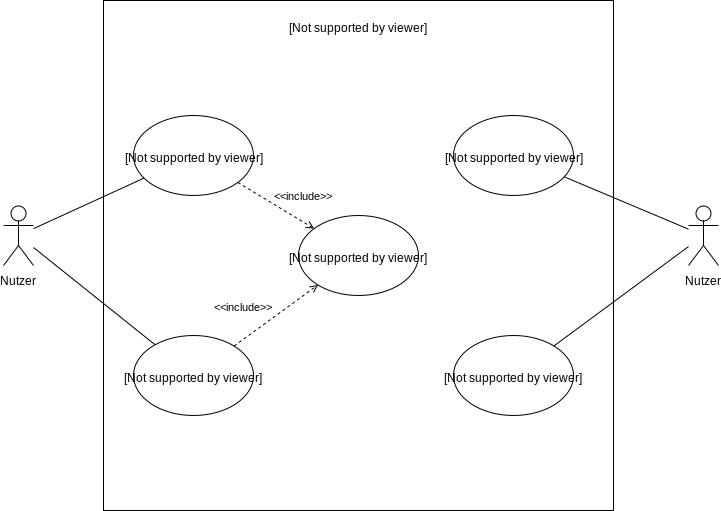
\includepdf[pages=-, scale=0.8, pagecommand={\section{Anwendungsfälle}\subsection{Client}}]{images/AFD_Client.pdf}
    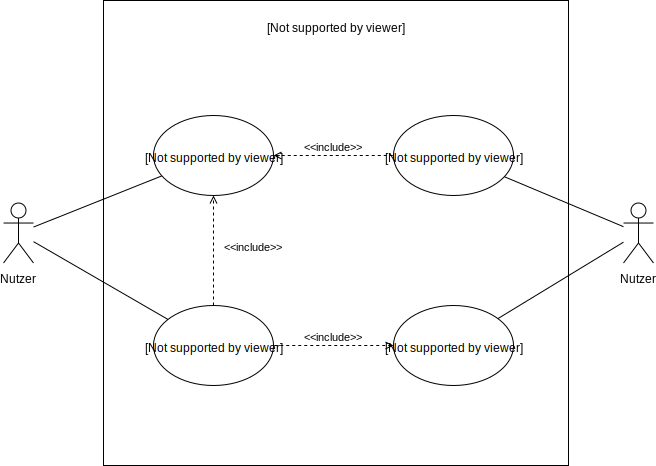
\includepdf[pages=-, scale=0.8, pagecommand={\subsection{Editor}}]{images/AFD_Editor.pdf}
    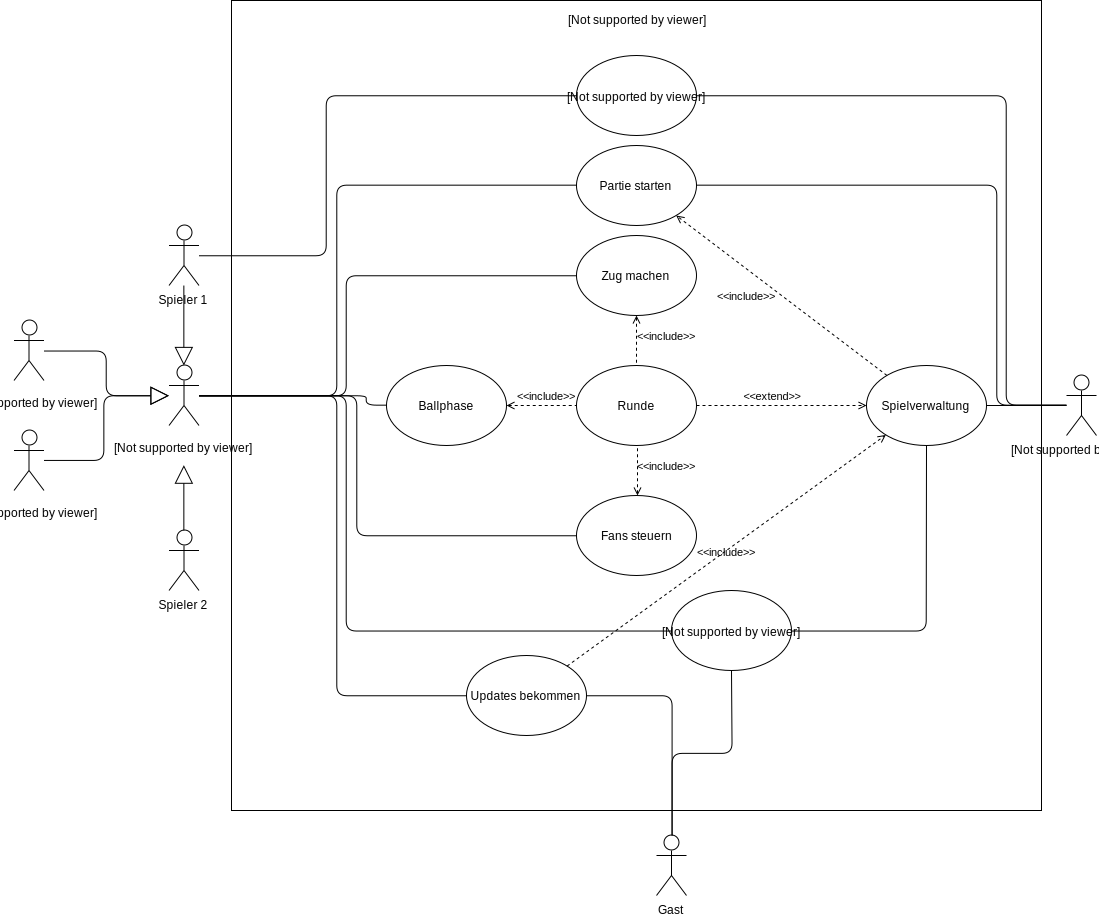
\includepdf[pages=-, scale=0.8, pagecommand={\subsection{Partie}}]{images/AFD_Party.pdf}
    \includepdf[pages=-, scale=0.8, pagecommand={\section{Abläufe im System}\subsection{State-Machine Server}}]{images/SM_Server.pdf}
    \includepdf[pages=-, scale=0.8, pagecommand={\subsection{State-Machine Client Netzwerk}}]{images/SM_ClientAnmelden.pdf}
    \includepdf[pages=-, scale=0.8, pagecommand={\subsection{State-Machine Client}}]{images/Client_SM.pdf}
    \includepdf[pages=-, scale=0.8, pagecommand={\subsection{State-Machine Rundenablauf}}]{images/SM_Rundenablauf.pdf}
    \includepdf[pages=-, scale=0.7, pagecommand={\subsection{Sequenzdiagramm Spielerphase}}]{images/SD_Spielerphase.pdf}
    \includepdf[pages=-, scale=0.8, pagecommand={\subsection{Sequenzdiagramm Fanphase}}]{images/SD_Fanphase.pdf}
\end{document}
